\begin{landscape}
\section{Anexo de diagramas}

    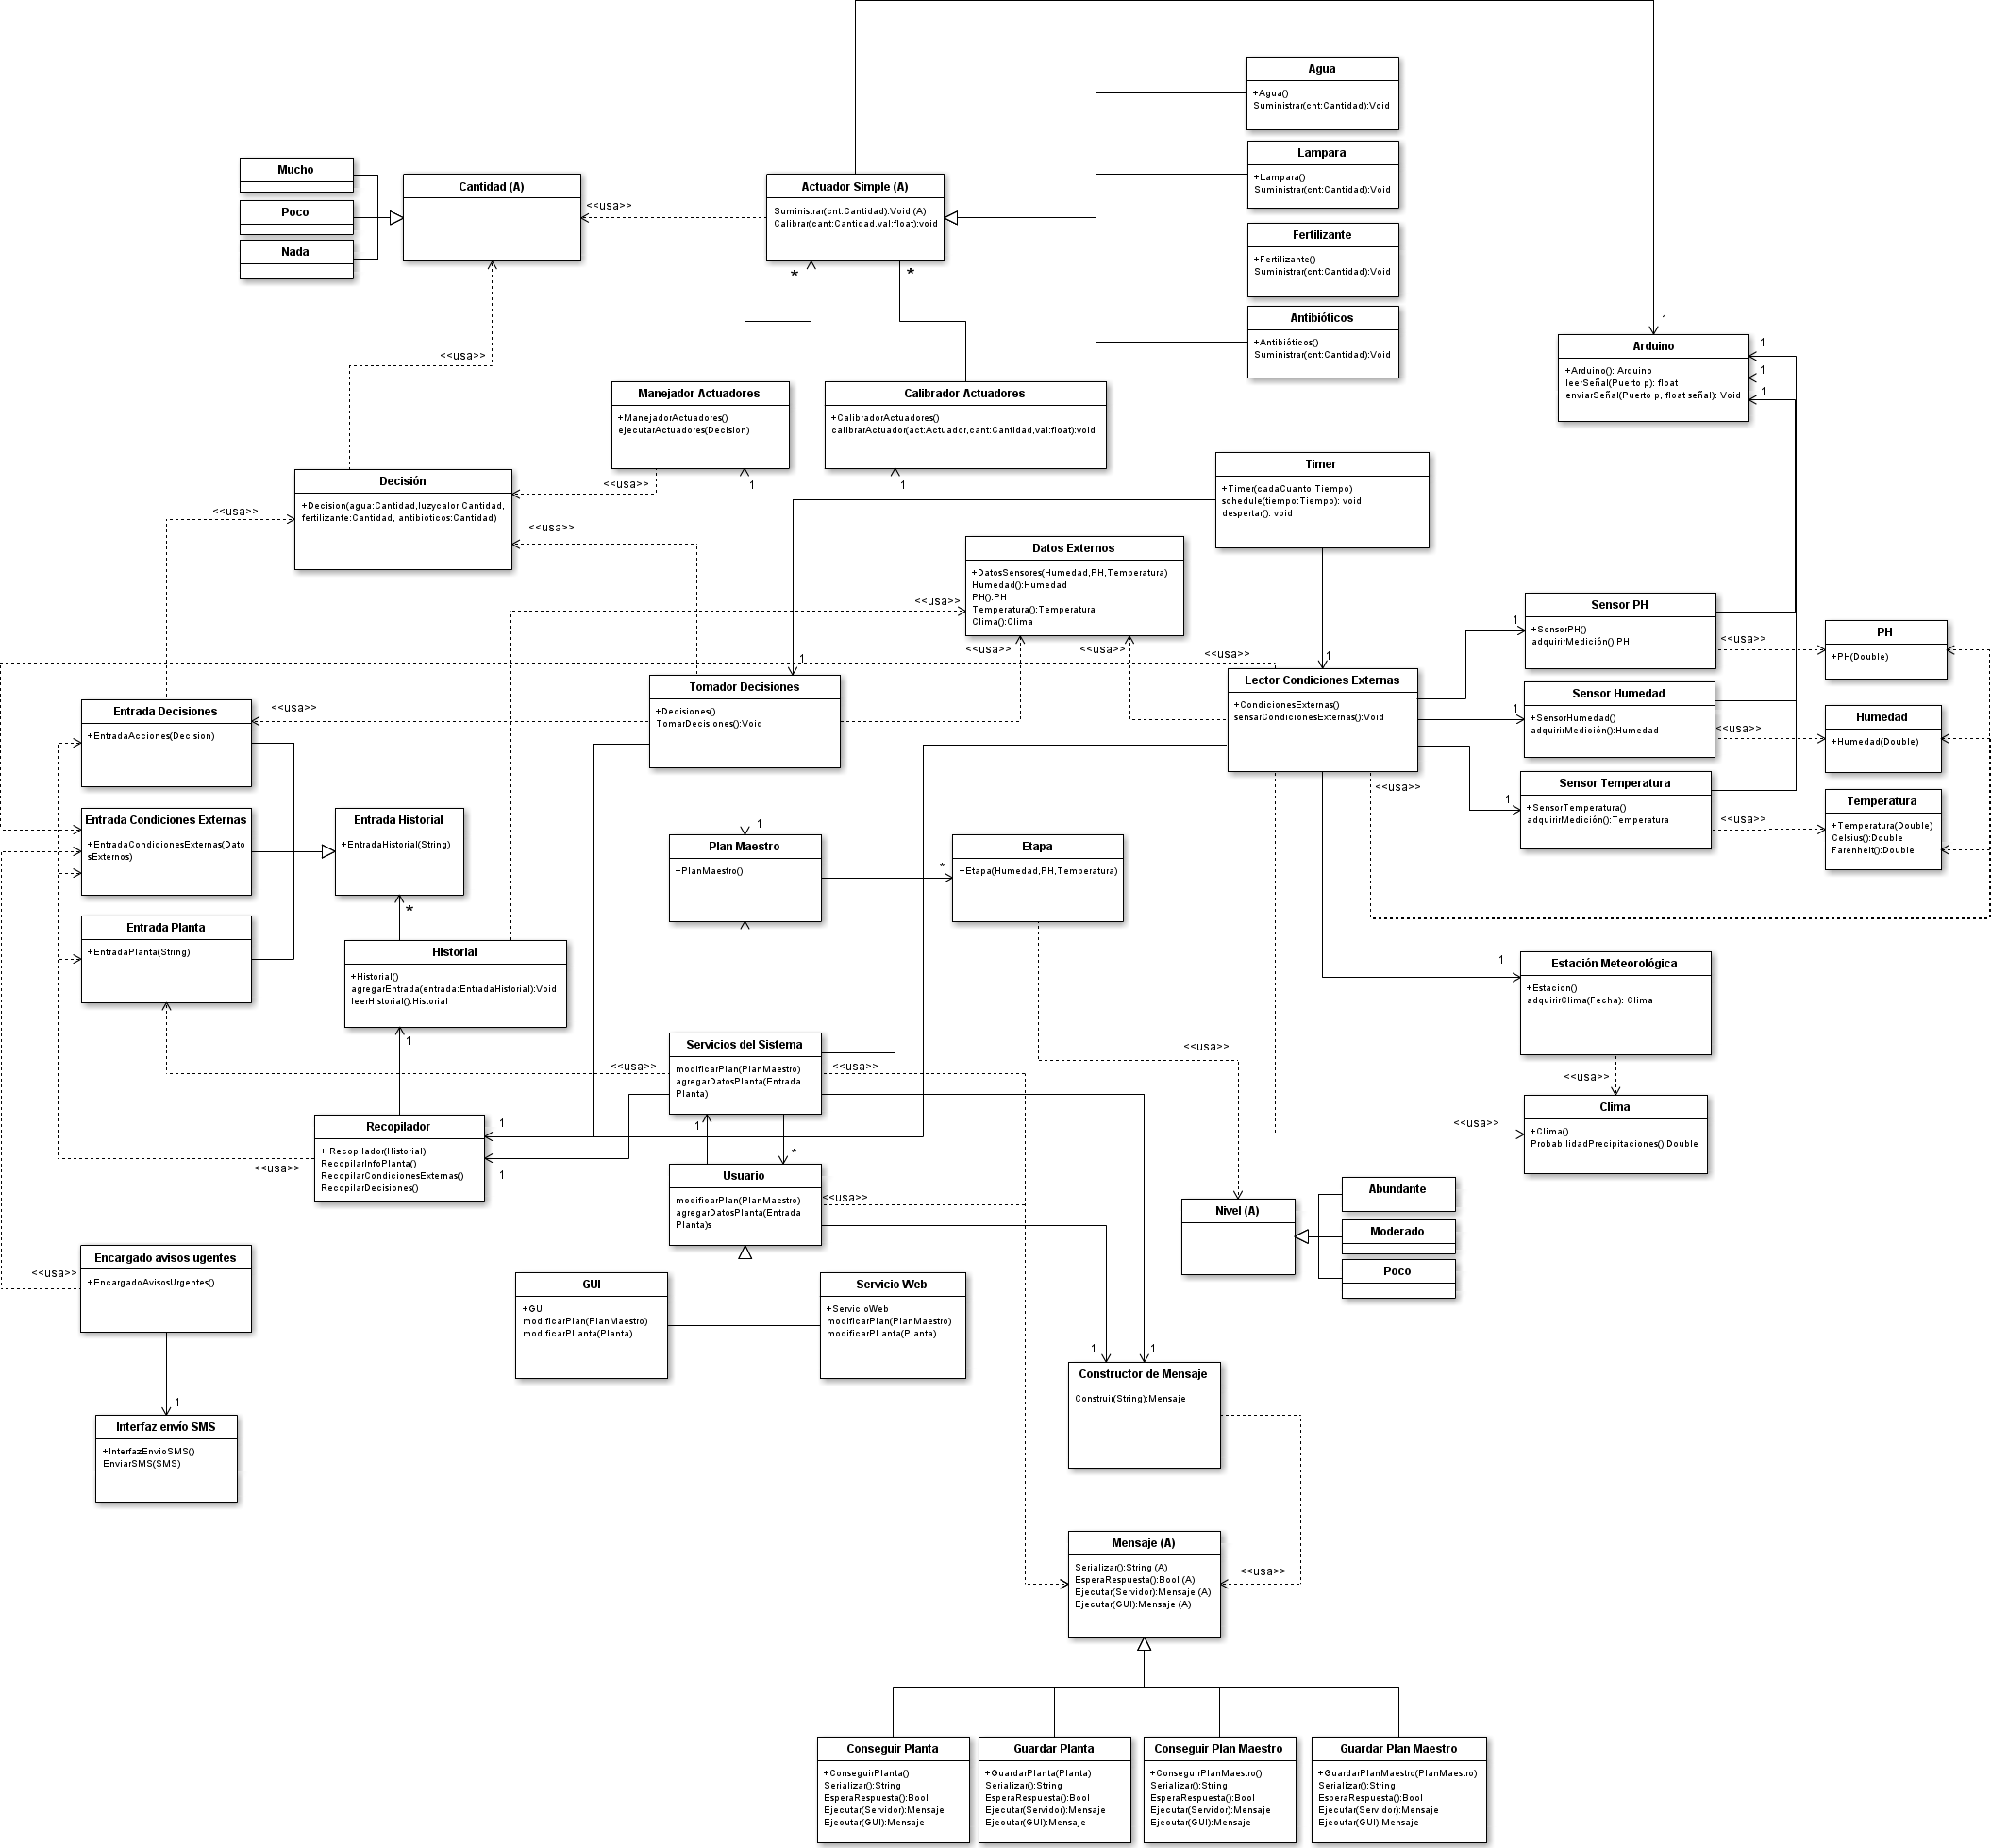
\includegraphics[width=0.9\textwidth]{img/clases.png}
    \centerline{ \small \scshape Diagrama de clases.}

    \hfill

    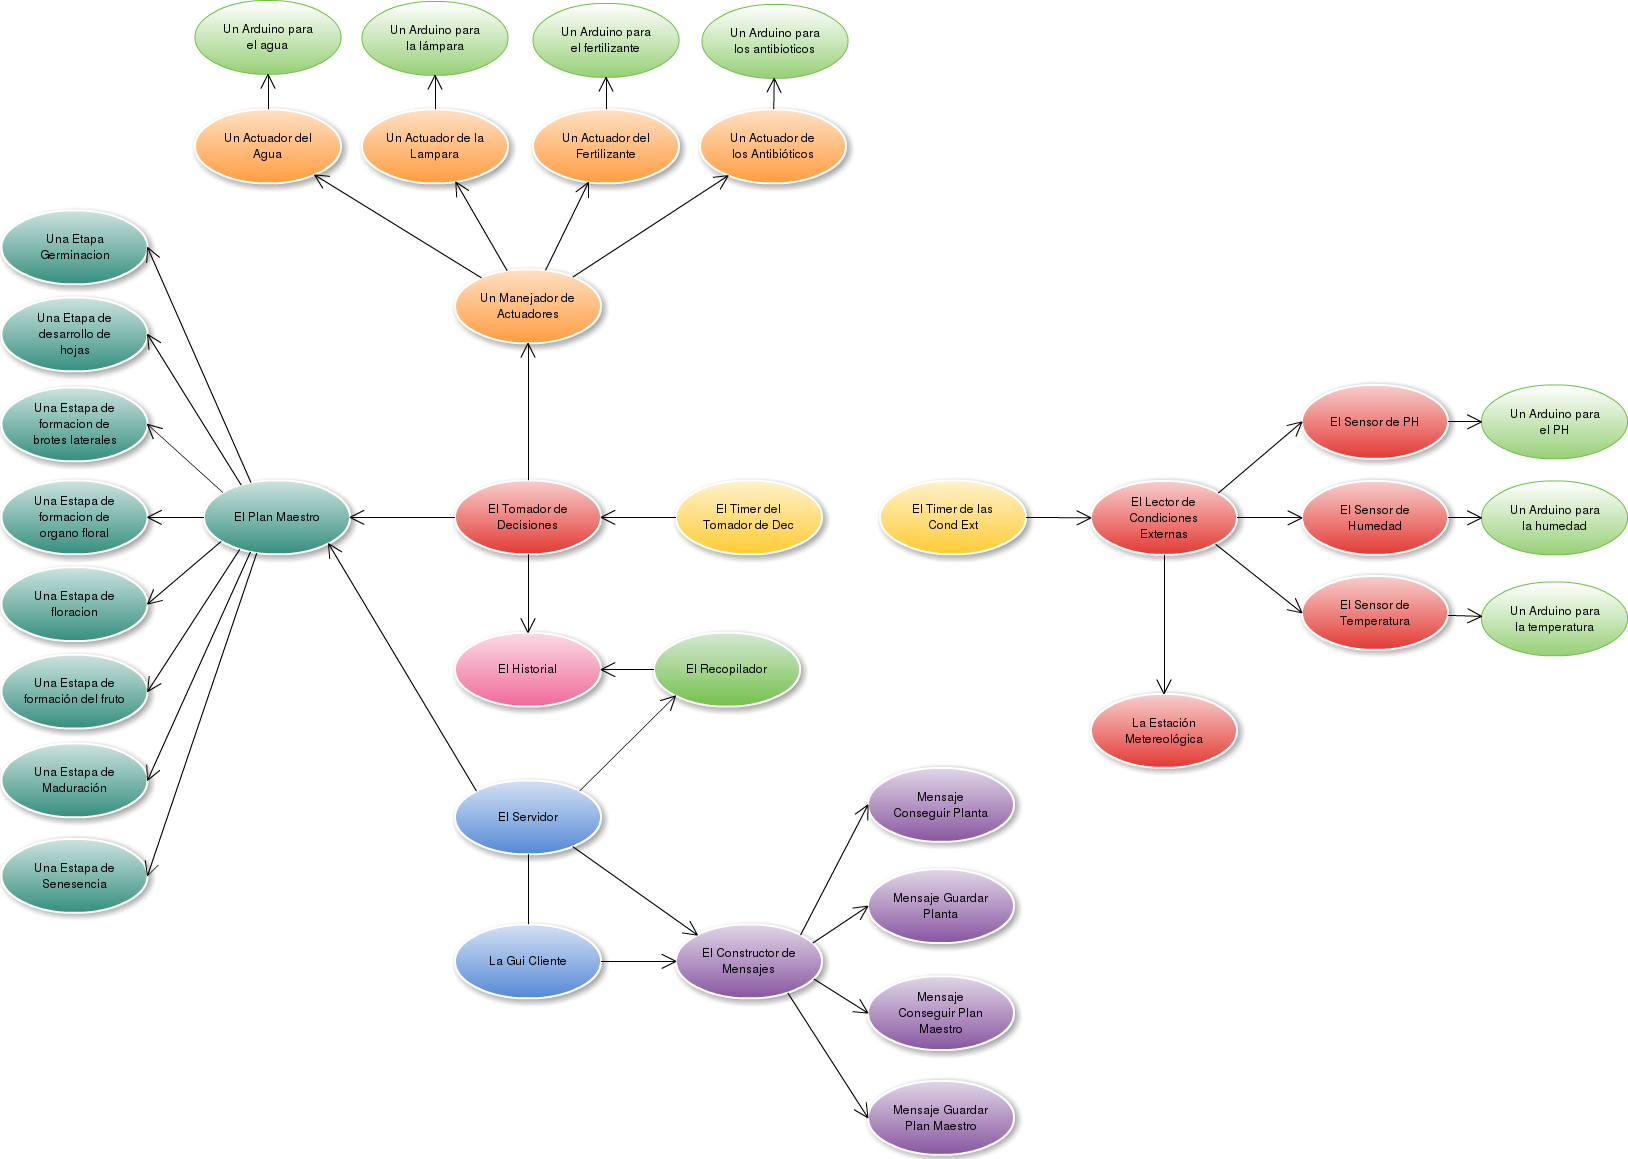
\includegraphics[width=1.2\textwidth]{img/objetosGeneral.png}
    \centerline{ \small \scshape Diagrama de objetos sin \historial{}.}

    \hfill

    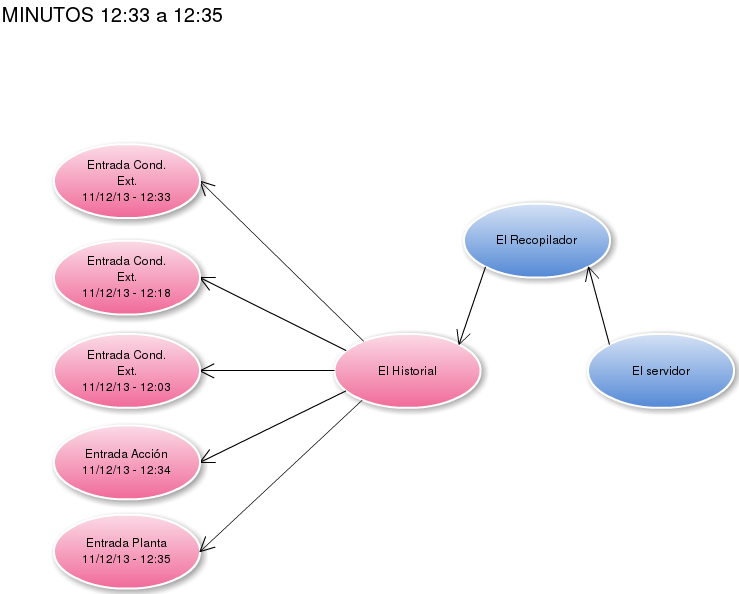
\includegraphics[width=0.5\textwidth]{img/objetosHistorial.png}
    \centerline{ \small \scshape Diagrama de objetos de \historial{}.}

    \hfill

    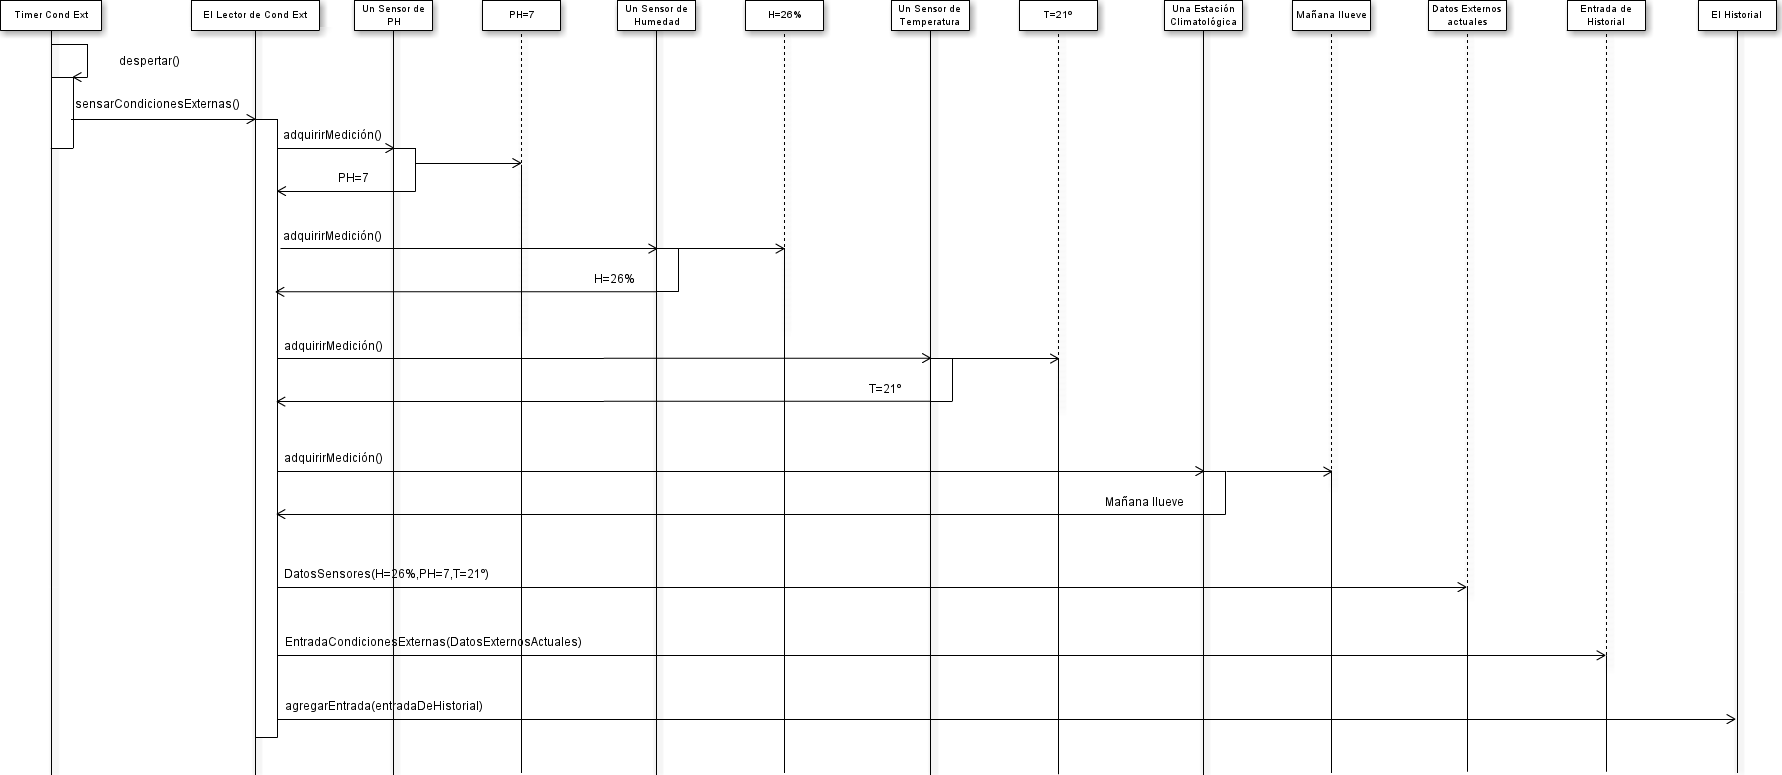
\includegraphics[width=1.2\textwidth]{img/condicionesExternas.png}
    \centerline{ \small \scshape Diagrama de secuencia \condiciones{}.}

    \hfill

    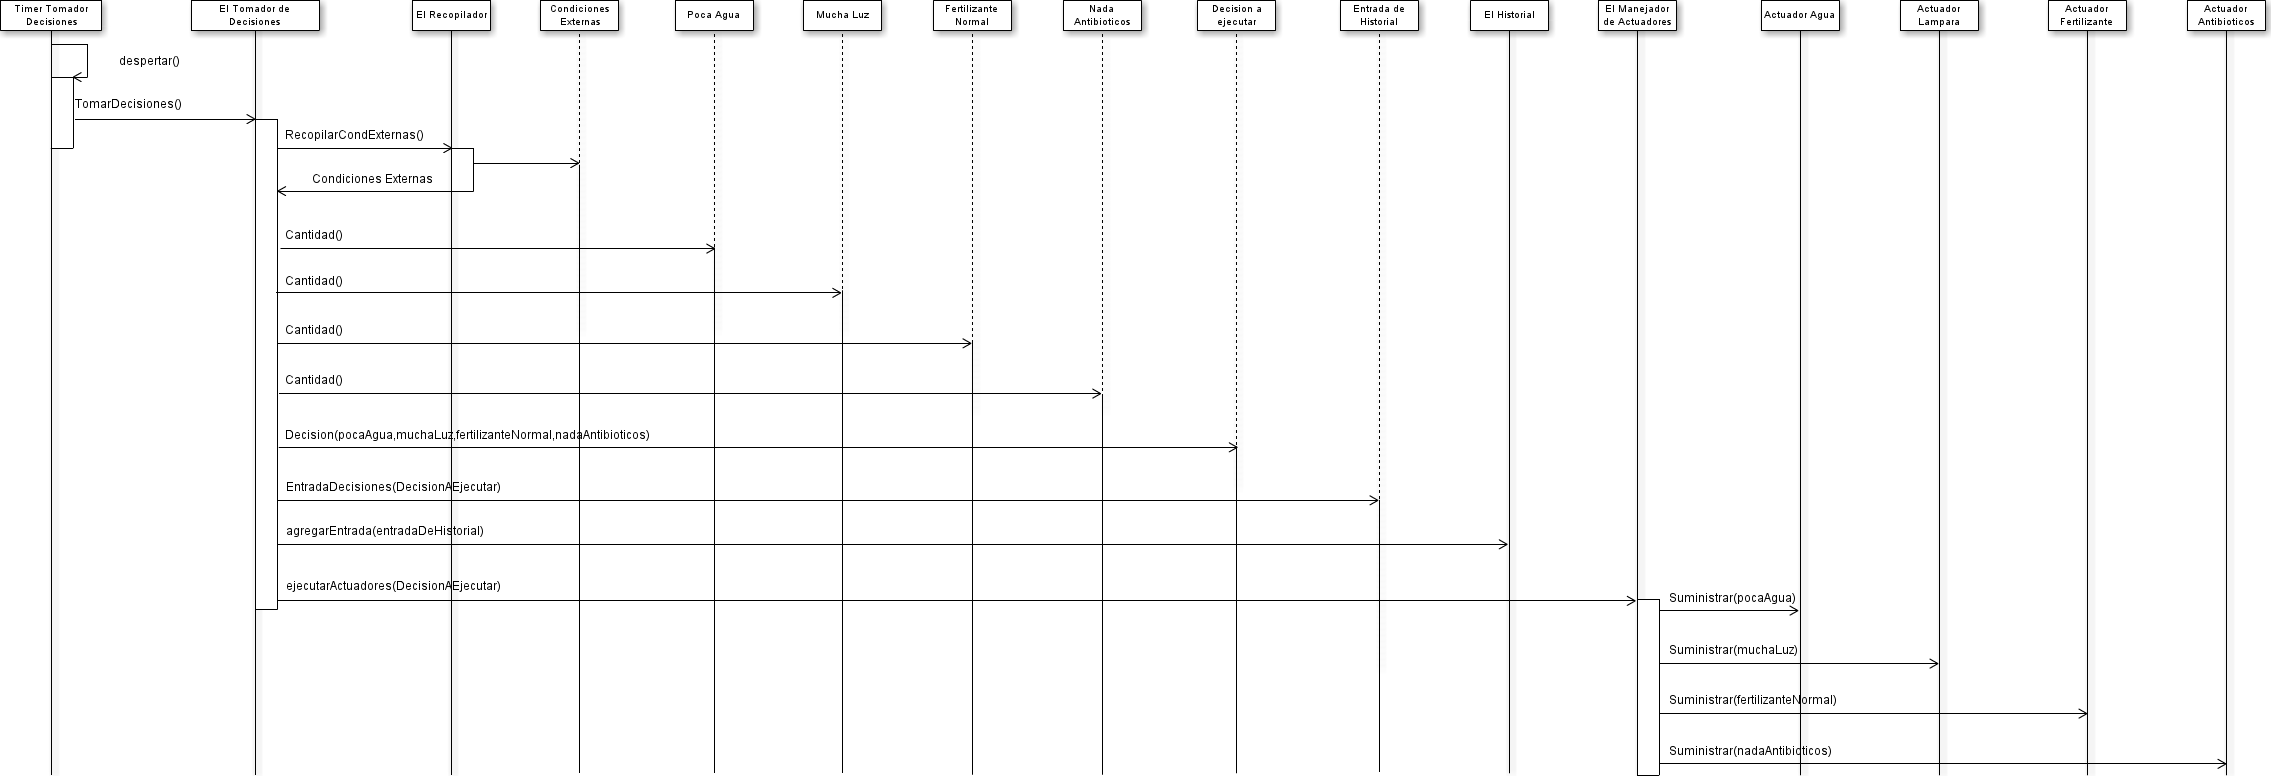
\includegraphics[width=1.3\textwidth]{img/decisiones.png}
    \centerline{ \small \scshape Diagrama de secuencia \decisiones{}.}


\end{landscape}
